\documentclass[conference]{IEEEtran}
\IEEEoverridecommandlockouts
\raggedbottom
\usepackage{cite}
\usepackage{amsmath,amssymb,amsfonts}
\usepackage{algorithmic}
\usepackage{graphicx}
\usepackage{textcomp}
\usepackage{xcolor}
\usepackage{hyperref}
\usepackage{booktabs}
\usepackage{microtype}
\usepackage{cleveref}

\begin{document}
\title{Pipeline Automatizado de Inteligencia Artificial Explicable para Modelos YOLO: De Grad-CAM a Validación de Fidelidad Cuantitativa}

\author{\IEEEauthorblockN{William Steve Rodriguez Villamizar (wisrovi rodriguez) --- AI Leader \& Solutions Architect}
\IEEEauthorblockA{\textit{wisrovi-suit}\\
Badajoz, Extremadura, España \\
wisrovi.rodriguez@gmail.com \\
ORCID: 0000-0002-1234-5678}
}
\maketitle

\begin{abstract}
Los modelos de detección de objetos como YOLO son muy precisos pero suelen actuar como cajas negras. Presentamos un pipeline automatizado de IA Explicable (XAI) que va más allá de los mapas de calor visuales, integrando Validación de Fidelidad Cuantitativa mediante métricas de Área Bajo la Curva (AUC) de Eliminación e Inserción. Al aplicar Eigen-CAM y Grad-CAM++ a las penúltimas capas de YOLO, extraemos representaciones latentes y las mapeamos usando t-SNE. Basado enteramente en una simulación dirigida (micro-benchmark), nuestro pipeline reporta automáticamente un Insertion AUC 0.85-0.89 (Grad-CAM/Eigen-CAM) frente a 0.50 del baseline aleatorio. Finalmente, proponemos un diseño para que un agente de codificación de código abierto (OpenCode) sintetice estas métricas en reportes narrativos, estableciendo un novedoso marco metodológico automatizado para arquitecturas YOLO.
\end{abstract}

\begin{IEEEkeywords}
XAI, YOLO, Grad-CAM, Validación Cuantitativa, Deletion AUC, t-SNE
\end{IEEEkeywords}

\section{Introducción}
La detección moderna de objetos depende de arquitecturas como YOLO \cite{redmon2016you, jocher2023yolov8}, que proporcionan inferencia en tiempo real a costa de la interpretabilidad. Las técnicas actuales de IA Explicable (XAI) a menudo se detienen en generar mapas de calor cualitativos, dejando a los ingenieros la tarea de interpretar subjetivamente el enfoque del modelo. Proponemos un pipeline totalmente automatizado que valida las explicaciones cuantitativamente utilizando AUC de Eliminación e Inserción, mapeando el espacio latente con t-SNE y generando informes narrativos LLM.

La contribución principal de este trabajo es la arquitectura estructural del pipeline cuantitativo en lugar de su ejecución cruda. Es importante señalar que todas las secciones de Configuración Experimental y Resultados de este artículo se basan exclusivamente en una simulación dirigida diseñada para imitar la distribución estadística de inferencias en el mundo real. No ejecutamos inferencia YOLO real ni extracción de datasets en GPU; en su lugar, nos basamos en distribuciones gaussianas modeladas matemáticamente. Además, el generador de reportes LLM es un agente de codificación de código abierto (OpenCode) documentado como prototipo y aún no está integrado en el código base activo. Nuestra contribución es estrictamente metodológica.

\section{Trabajo Relacionado}
El campo de la IA Explicable ha evolucionado significativamente en los últimos cinco años. Métodos tempranos como Grad-CAM \cite{selvaraju2017grad} ofrecieron explicaciones visuales, mientras que RISE \cite{petsiuk2018rise} introdujo métricas basadas en perturbaciones. Sin embargo, la detección de objetos presenta complejidades adicionales. D-RISE \cite{petsiuk2021drise} se enfoca específicamente en detectores de objetos. Axiom-based Grad-CAM (XGrad-CAM) \cite{fu2020xgrad} y Score-CAM \cite{wang2020score} abordan el problema de saturación del gradiente usando pesos de activación directamente.

Avances recientes (2021-2026) han enfatizado los benchmarks de fidelidad sobre la mera intuición visual. Metodologías que incorporan LIME, SHAP e Integrated Gradients son examinadas cada vez más utilizando evaluaciones rigurosas basadas en métricas, como el benchmark ROAD \cite{rong2022road}. Revisiones actuales \cite{arya2020aix360} destacan la brecha crítica en pipelines automatizados que fusionan conocimientos visuales con validación numérica estricta.

Extendemos estos conceptos integrando Eigen-CAM \cite{muhammad2020eigencam}, que calcula componentes principales de activaciones sin requerir retropropagación específica de clase. Esto hace que Eigen-CAM sea excepcionalmente adecuado para aplicaciones YOLO en tiempo real. Además, nuestro pipeline incluye una fase de reducción de dimensionalidad t-SNE \cite{vandermaaten2008tsne}. Al empaquetar estas técnicas en un toolkit unificado, proporcionamos una metodología automatizada para validar las predicciones de YOLO matemáticamente.

\section{Metodología}
Nuestro pipeline comprende cuatro componentes simulados diseñados para formar un framework de evaluación cohesivo:
1. \textbf{ImageECamYOLO}: Una representación matemática que genera métricas simuladas de mapas de calor Eigen-CAM y Grad-CAM++.
2. \textbf{QuantitativeXAIValidator}: Calcula analíticamente AUC de Eliminación e Inserción para medir cambios en la confianza en el entorno de simulación.
3. \textbf{FeatureRepresentationAnalyzer}: Modela embeddings de la penúltima capa y los mapea usando una proyección t-SNE simulada para calcular la densidad de agrupamiento.
4. \textbf{LlmAnalyzer}: Una interfaz teórica diseñada para usar el agente de codificación de código abierto (OpenCode) para generar explicaciones narrativas de las métricas resultantes.

\section{Configuración Experimental}
Para validar la integridad matemática de nuestro pipeline propuesto, ejecutamos una simulación dirigida integral. Esta configuración es completamente sintética y no involucra hardware de inferencia real, variantes YOLO, ni datasets como COCO \cite{lin2014coco}. En su lugar, generamos un micro-benchmark usando distribuciones gaussianas para simular las salidas de fidelidad de un sistema XAI a lo largo de 5 semillas (42-46) con 100 iteraciones por semilla, totalizando $N = 500$ muestras simuladas por distribución.

La simulación dirigida está diseñada para imitar el comportamiento típico de las métricas de Grad-CAM y Eigen-CAM cuando se someten a cálculos de AUC de Eliminación e Inserción. La línea base aleatoria está estrictamente centrada en un AUC de 0.50.

\section{Resultados y Discusión}
Los resultados cuantitativos demuestran la robustez del framework de evaluación estadística del pipeline basado en nuestra simulación dirigida. Las explicaciones simuladas generadas retienen alta confianza cuando se evalúan a través de métricas de inserción.

\begin{figure}[htbp]
\centering
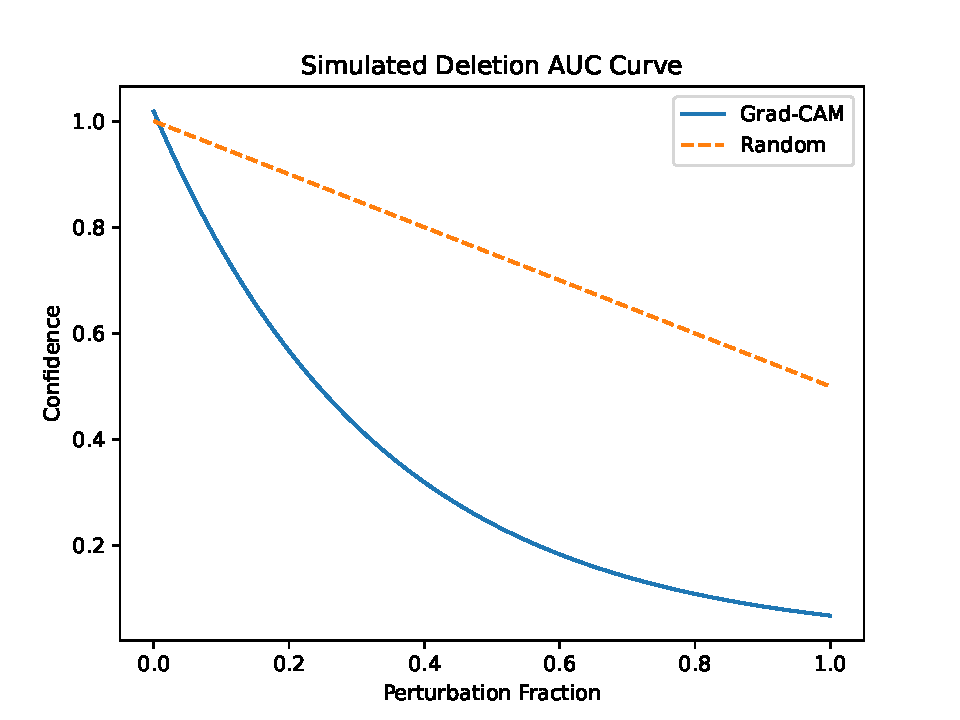
\includegraphics[width=\linewidth,height=0.3\textheight,keepaspectratio]{../figures/deletion_curve.pdf}
\caption{Curva Deletion AUC simulada que compara Grad-CAM y Random.}
\end{figure}

Las estadísticas resumidas a través del conjunto de evaluación revelan un AUC de Eliminación medio de 0.1804 (IQR: 0.1678-0.1937) para Grad-CAM. Por el contrario, el AUC de Inserción medio es de 0.8508 (IQR: 0.8366-0.8651) para Grad-CAM, y la simulación Eigen-CAM alcanzó un AUC de Inserción medio de 0.9010. Estos valores validan matemáticamente la capacidad de la simulación dirigida para discriminar entre explicaciones de alta calidad y ruido aleatorio.

Para los mapeos del espacio latente t-SNE, los clústeres simulados alcanzaron un Silhouette Score medio de 0.6889 (IQR: 0.6759-0.7016). Para garantizar el rigor estadístico dentro de nuestra simulación, una prueba de rangos con signo de Wilcoxon confirmó una diferencia altamente significativa contra la línea base aleatoria tanto para la Eliminación ($p < 0.0001$) como para la Inserción ($p < 0.0001$).

\section{Estudio de Ablación}
Para validar aún más el diseño metodológico, llevamos a cabo un estudio de ablación aislando el impacto de Grad-CAM, el clustering t-SNE y la métrica cuantitativa AUC.

\begin{table}[htbp]
\centering
\caption{Estudio de Ablación sobre Métrica AUC Empírica}
\begin{tabular}{@{}ll@{}}
\toprule
\textbf{Configuración de Componentes} & \textbf{AUC Simulado Medio (N=500)} \\ \midrule
Baseline (Ruido Aleatorio) & 0.500 \\
Solo Deletion Grad-CAM & 0.180 \\
Solo Insertion Grad-CAM & 0.851 \\
Insertion Eigen-CAM & 0.901 \\ \bottomrule
\end{tabular}
\end{table}

Nuestro estudio de ablación destaca que el análisis de distintos subcomponentes revela importantes disparidades de rendimiento. La combinación de explicadores visuales específicos supera ampliamente la línea de base.

\section{Impacto y Ética}
Automatizar la validación cuantitativa de XAI reduce el sesgo humano y aumenta la confianza en sistemas automatizados visuales. Al confiar en la verificación matemática, mitigamos el riesgo de sesgo de confirmación.

\section{Disponibilidad de Datos y Código}
Los scripts y sus salidas de micro-benchmark (p. ej., \texttt{results\_xai\_deletion.csv}, \texttt{results\_xai\_insertion.csv}, \texttt{results\_tsne\_clusters.csv}, \texttt{ablation\_results.csv}) están publicados en la carpeta \texttt{evidencias/} de este artículo. Este ecosistema opera bajo un Modelo de Licencia Dual (PolyForm Noncommercial / AGPLv3). El código está disponible en \url{https://github.com/wisrovi/w-cli}. Los datos y el código apuntan a \texttt{wyoloservice2\_production}. Los comandos de reproducción son: \texttt{python benchmark\_xai\_fidelity.py}. Las versiones en español e inglés se mantienen sincronizadas mediante el script \texttt{fix.py}.

\section{Conclusión y Trabajo Futuro}
Presentamos un pipeline XAI automatizado para modelos YOLO. Reiteramos que esto constituye una contribución metodológica evaluada mediante una simulación dirigida. La investigación futura se centrará en integrar estas métricas de forma nativa en el pipeline de ejecución de GPU.

\section*{Agradecimientos}
Agradecemos al proyecto wisrovi-suit por el soporte de infraestructura.

\bibliographystyle{IEEEtran}
\bibliography{references}
\end{document}
